\chapter{Web aplikacija}

Svi podaci koji su pohranjeni u bazi podataka trebaju biti korisnicima na raspolaganju jednostavno i intuitivno. U tu je svrhu kreirana aplikacija radi prikaza i vizualizacije podataka korisnicima u stvarnom vremenu. Web aplikacija treba biti javno dostupna na internetu kako bi korisnici razvijenog sustava mogli pregledavati podatke poslane s uređaja. Za objavu web aplikacije na internet \engl{deployment} kreirani su vlastiti resursi na kojima se izvršava aplikacija. Za infrastrukturu aplikacije korišteni su resursi platforme AWS koji pružaju iznajmljivanje virtualnih računala te se na njima mogu pokrenuti vlastite računalne aplikacije. Za web aplikaciju koja će korisnicima pružati uvid u podatke odabrana je Grafana koja nudi brojne funkcionalnosti za vizualizaciju podataka. Nadalje, kreiran je i alarmni sustav koji obavještava o promjenama stanje koja dolaze od uređaja. 

\section{Infrastruktura aplikacije}

Temelj cijele infrastrukture aplikacije jest usluga Amazon EC2 \engl{Elastic Compute Cloud}. Ova usluga pruža skalabilni računalni kapacitet na zahtjev u oblaku platforme AWS. Ova usluga omogućava pokretanje neograničenog broja virtualnih poslužitelja, ovisno o zahtjevima aplikacije i razvijanog sustava, konfiguriranje sigurnosti i umrežavanja te upravljanje pohranom. Usluga EC2 nudi razne prednosti \cite{aws_docs}:
\begin{itemize}
	\item fleksibilno skaliranje: omogućava brzo povećanje ili smanje kapaciteta u kombinaciji s uslugom EC2 Auto Scaling za automatsko skaliranje radi prilagodbe troškova,
	\item potpuna kontrola nad instancom: pruža pristup instanci kao i bilo kojem stroju, moguće pokretanje i zaustavljanje spajanjem na udaljeno računalo, ali i API pozivom,
	\item fleksibilne usluge objave u oblaku: nudi izbor između više vrsta instanci, operacijskih sustava i softverskih paketa te nudi konfiguraciju memorije, procesora i pohrane,
	\item integracija s drugim uslugama: jednostavno se integrira s ostalim uslugama us sklopu platforme AWS,
	\item pouzdanost: nudi vrlo pouzdano okruženje u kojem se zamjenske instance mogu brzo pokrenuti, te je obaveza ugovora o razini usluge Amazon EC2 \engl{Service Level Agreement - SLA} dostupnost od 99,99\% za svaku regiju,
	\item sigurnost: arhitektura nudi različite sigurnosne značajke i postavljanje virtualnih privatnih mreža za ograničen pristup resursima.
\end{itemize}

EC2 instance virtualni su poslužitelji koji rade na infrastrukturi računalstva u oblaku tvrtke Amazon. Jedan fizički AWS poslužitelj uslužuje više EC2 virtualnih poslužitelja koje pokreće hipervizor na računalu domaćinu. Ova usluga pružanja virtualne infrastrukture dio je skupa IaaS usluga koje AWS nudi. EC2 virtualni poslužitelji kopije su izvornog predloška na kojem se temelje. AMI \engl{Amazon Machine Image} temeljna je komponenta koja omogućava pokretanje virtualnih poslužitelja u AWS infrastrukturi. Predstavlja virtualni stroj koji sadrži sve potrebne informacije za pokretanje instance, uključujući operacijski sustav, aplikacije te konfiguracijske podatke. To je prilagodljivi predložak za EC2 instance. Iz jednog AMI predloška, odnosno slike stroja, moguće je kreirati više istih EC2 instanci, što olakšava njihovo stvaranje i objavu na internet. Ovo je korisno za horizontalno skaliranje aplikacija. Slika \ref{fig:ami} prikazuje način na koji funkcionira AMI predložak - kreira instance bilo koje vrste te ih pokrene na domaćinskim računalima \cite{ec2}.

\begin{figure}[ht]
	\centering
	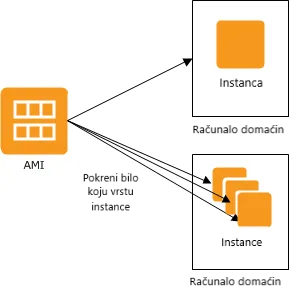
\includegraphics[scale=0.6]{imgs/ami}
	\caption{AMI predložak i distribucija slika stroja na instance \cite{ec2}}
	\label{fig:ami}
\end{figure}

AMI predlošci podržavaju dva tipa virtualizacije: hardversku virtualizaciju i paravirtualizaciju. Predložak s hardverskom virtualizacijom pruža mogućnost pokretanja operacijskog sustava izravno na vrhu virtualnog stroja bez ikakvih izmjena, kao da se pokreće na samom hardveru \engl{bare-metal hardware}. Domaćinski sustav usluge EC2 emulira dio ili sav temeljni hardver koji je predstavljen gostu odnosno AMI slici. Moguće je isto tako koristiti hardverska proširenja koji pružaju brzi pristup domaćinskom hardveru. Paravirtualizacija koristi poseban pokretački program koji lančano učitava jezgru u AMI sliku. Paravirtualni gosti mogu se pokretati na domaćinskom hardveru koji nema eksplicitnu podršku za virtualizaciju. Ovaj tip ne simulira hardver, nego pravi hiperpozive \engl{hypercalls} za izvršavanje osjetljivih CPU naredbi. Preporuča se odabir hardverske virtualizacije, iako generalno paravirtualizacija pruža bolje performanse, zbog poboljšanja hardverske virtualizacije i novih upravljačkih programa koji izjednačava rad obje vrste virtualizacije. 

Pri kreiranju instance potrebno je definirati i njezinu vrstu. Vrsta koja se navede određuje hardver dostupan instanci. Svaka vrsta nudi različitu ravnotežu računalnih, memorijskih i mrežnih resursa. Vrste su grupirane u skupine na temelju potreba ciljnih aplikacija. AWS pruža sljedeće vrste instanci:
\begin{itemize}
	\item opće namjene \engl{general purpose}, 
	\item optimiziranog računanja \engl{compute optimized},
	\item optimizirane memorije \engl{memeory optimized},
	\item optimizirane pohrane \engl{storage optimized}, 
	\item ubrzanog računanja \engl{accelerated computing},
	\item računanja visokih performansi \engl{high-performance computing}.
\end{itemize}

Vrstu instance potrebno je odabrati na temelju zahtjeva same aplikacije. Isto tako, pri kreiranju instance, uvijek je potrebno voditi računa o odabiru regije - optimalno je odabrati regiju kojoj je klijentski promet najbliži.

Za potrebe razvijenog sustava, kreirana je EC2 instanca opće namjene s najmanjim resursima budući da je klijentski promet jako malen, odnosno vrlo malo korisnika pristupa aplikaciji. Također, pridružena joj je instanca spremnika za pohranu veličine 8 GB. Operacijski sustav na kreiranoj instanci aplikacije jest Linux radi lakšeg spajanja na instancu i pokretanja web aplikacije putem komandne linije. Pri stvaranju instance kreirana je nova sigurnosna grupa koja omogućava spajanje na virtualno računalo putem SSH klijenta.

Instanci je automatski dodijeljena virtualna privatna mreža \engl{Virtual Private Cloud - VPC} koja predstavlja izolirani virtualni mrežni prostor unutar AWS infrastrukture. Omogućava potpunu kontrolu nad mrežnim okruženjem, uključujući izbor vlastitog IP adresnog prostora, konfiguraciju podmreža, postavljanje usmjeravanja i pristupnih kontrola mreže. Svaka je virtualna privatna mreža podijeljena na manje dijelove mreže zvane podmreže. One mogu biti privatne ili javne te se automatski za svaku mrežu kreiraju tri podmreže. Svaka je kreirana podmreža prema zadanim postavkama privatna, te je za pristup instanci odnosno aplikaciji koja se nalazi za njom potreban javni pristup. Iako omogućavanje javnog pristupa znači da svatko može pristupiti IP adresi instance s interneta, unošenje IP adrese pri svakom pristupu aplikaciji nije prilagođeno korisniku, što narušava korisničko iskustvo korištenja aplikacije. Stoga je potrebno uvesti komponentu za balansiranje opterećenja \engl{load balancer}. Balanseri preusmjeravaju korisničke zahtjeve na manje opterećene instance i tako ravnomjerno raspoređuju ulazni promet. Budući da je u razvijenom sustavu korištena samo jedna instanca na kojoj se pokreće aplikacija, ovdje je primarna svrha balansera pružiti DNS naziv koji će biti javno dostupan korisnicima, i tako poboljšati iskustvo korištenja aplikacije. 

Aplikacijskoj instanci potrebno je dodijeliti pravila za ulazne zahtjeve, odnosno omogućiti TCP komunikaciju s podmreže u kojoj se nalazi balanser. Tim se pravilom omogućuje prolaz zahtjeva s balansera prema aplikacijskoj instanci. Isto tako, iz sigurnosnih razloga poželjno je koristiti protokol HTTPS za pristup balanseru. Za korištenje protokola HTTPS potrebno je učitati certifikat, no budući da domena na kojoj se nalazi balanser nije službeno registrirana, ne posjeduje niti službeno potpisani certifikat. Stoga je lokalno kreiran samopotpisani certifikat pomoću biblioteke \textit{OpenSSL} i zatim učitan u oblak. Slika \ref{fig:load_balancer} prikazuje mrežnu povezanost balansera i instance na kojoj se nalazi aplikacija. Balanser sluša promet na vratima 443, što su vrata za protokol HTTPS. Dolazni zahtjevi prosljeđuju se skupini ciljnih instanci, ovdje pod nazivom \textit{GrafanaTargetGroup}, u kojoj se mogu nalaziti sve buduće stvorene instance na kojima se pokreće aplikacija. Nadalje, promet se prosljeđuje ciljnoj instanci koja je dostupna na vratima 3000. Na tim je istim vratima pokrenuta aplikacija. 

\begin{figure}[ht]
	\centering
	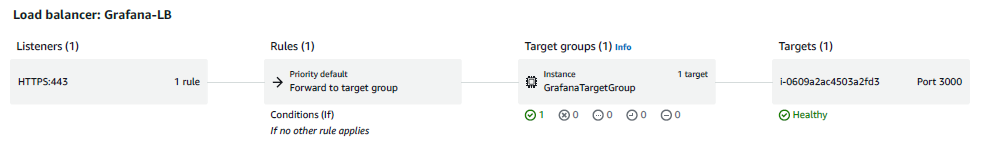
\includegraphics[scale=0.7]{imgs/load_balancer}
	\caption{Mrežna povezanost balansera i aplikacijske instance}
	\label{fig:load_balancer}
\end{figure}

Kako bi se maksimalno izoliralo izvođenje aplikacije i tako ostavilo prostora za izvršavanje drugih procesa na virtualnom računalu, na instanci EC2 aplikacija je pokrenuta pomoću alata Docker radi kontejnerizacije aplikacije. Sljedeći programski isječak prikazuje naredbu za preuzimanje i pokretanje Docker slike za Grafanu. Isto tako, potrebno je izložiti vrata na kojoj se pokreće aplikacija kako bi joj se moglo pristupiti. Grafana nudi dvije verzije - otvorenog koda i \textit{enterprise}, koja nudi više značajki. Za potrebe razvijenog sustava korištena je slika verzije otvorenog koda. Potrebno je također i postaviti varijable okoline za povezivanje s SMTP poslužiteljem \engl{Simple Mail Transfer Protocol}, koji će kasnije služiti za slanje e-pošte obavijesti. Korišten je poslužitelj koji dolazi uz uslugu Gmail tvrtke \textit{Google}, te je potrebno navesti aplikacijsku lozinku koja se može kreirati u Gmail računu.

\begin{lstlisting}[caption={Pokretanje Docker slike za Grafanu}, language=bash]
sudo docker run -d -p 3000:3000 --name grafana 
	-e "GF_SMTP_ENABLED=true" \
	-e "GF_SMTP_HOST=smtp.gmail.com:587" \
	-e "GF_SMTP_USER=gmail.address@gmail.com" \
	-e "GF_SMTP_PASSWORD=GeneratedPassord123" \
	grafana/grafana-oss
\end{lstlisting}

\section{Grafana}

Grafana je platforma otvorenog koda za vizualizaciju i analizu podataka koja omogućava korisnicima stvaranje interaktivnih i prilagodljivih nadzornih ploča \engl{dashboards}. Cilj platforme jest olakšati analize vremenskih nizova podataka te integrira podatke iz različitih izvora podataka \engl{data source}, što mogu biti različite baze ili sustavi. Nudi jednostavnu vizualizaciju pomoću različitih grafičkih elemenata, uključujući linijske, stupčaste i tortne grafove. Široko je korištena zbog svoje sposobnosti da prezentira podatke na intuitivan način, omogućujući korisnicima donošenje informiranih odluka na temelju stvarnim podataka u stvarnom vremenu. Također, Grafana nudi alarmni sustav koji se koristi za izvještavanje korisnika o promjenama u podacima \cite{grafana}. 

Grafana se najčešće koristi za nadzor infrastrukture, performansi aplikacija i poslovnih metrika. Često je korištena za praćenje stanja poslužitelja, mrežnog prometa i performansi aplikacija. Također se koristi u poslovnoj analitici za praćenje poslovnih metrika. Isto tako, Grafana je korisna za IoT sustave upravo zbog sposobnosti vizualizacije velike količine podataka u stvarnom vremenu. Količine podataka koje IoT uređaji generiraju moraju se analizirati kako bi se dobili uvidi u očitana mjerenja, zdravlje sustava, kao i same performanse uređaja. Upravo zbog jednostavnog povezivanja s više različitih izvora podataka, njome se ostvaruje središnje mjesto za praćenje i analizu podataka iz cijele IoT mreže. Koristeći interaktivne nadzorne ploče, moguće je pratiti očitanja sa senzora u stvarnom vremenu i kreirati mnoge vizualizacije ovisno o potrebama sustava. Također podržava složene upite i transformacije podataka, što omogućuje njihovu dubinsku analizu. Korištenjem grafičkih elemenata i filtriranja podataka, mogu se lako identificirati trendovi, obrasci i anomalije u podacima \cite{grafana_iot}.

Kako bi web aplikacija mogla prikazivati podatke iz baze InfluxDB, na Grafani je potrebno stvoriti izvor podataka koji će služiti kao spojnica aplikacije i baze. Kako bi Grafana koristila InfluxDB kao izvor, koristi se dodatak \engl{plugin} koji služi kao poveznica između dva sustava. Osim što omogućuje njihovo povezivanje na razini dohvaćanja podataka, istovremeno preslikava vremenske okvire odabrane u Grafani u stvarne vremenske točke koje baza može parsirati. Budući da se u bazi nalaze dvije kante, \textit{esp32data} i \textit{esp32state}, za svaku je od njih potrebno napraviti poseban izvor podataka. Kako bi se Grafana uspješno spojila na bazu, potrebno je korisničko ime i lozinka, kao i token koji će omogućavati čitanje iz baze. U bazi InfluxDB kreiran je novi korisnik \textit{grafana} koji služi samo za potrebe web aplikacije i generirana su dva tokena, svaki za jednu kantu. Tokeni omogućavaju isključivo čitanje iz kante. Važno je također napomenuti kako se novi korisnici ne mogu kreirati putem sučelja baze InfluxDB, nego je potrebno lokalno preuzeti alat za upravljanje bazom te se udaljeno putem komandne linije spojiti na bazu InfluxDB i tako kreirati korisnika.

Za kreiranje upita prema bazi koristi se jezik Flux. To je skriptni jezik za podatke \engl{functional data scripting language} namijenjen postavljanju upita i analizi podataka vremenskih serija. Upiti mogu sadržavati agregacije i transformacije. Iako jezik dolazi sa predefiniranim skupom funkcija za rad nad vremenskim serijama, moguće je definirati i vlastite prilagođene funkcije. Većina upita u jeziku Flux prate jednaki slijed koji se lančano izvodi:
\begin{enumerate}
	\item definiranje izvora,
	\item filtriranje,
	\item oblikovanje,
	\item obrada. 
\end{enumerate}

Prvi korak je odabir izvora podataka, što se odnosi na izbor kante. Podaci su vraćeni u tabličnom obliku. Funkcije filtriranja iteriraju po svim redovima dobivene tablice i provjeravaju zadovoljavaju li unosi tražene kriterije. Primarne funkcije za filtriranje su \lstinline|range()| i \lstinline|filter()|. Prva funkcija filtrira podatke na temelju vremenskog okvira, dok \lstinline|filter()| filtrira vrijednosti na temelju sadržaja redaka. Koristi se predikatna funkcija definirana unutar izraza za evaluaciju retka. Svaki se redak predikatnoj funkciji prosljeđuje kao zapis koji sadrži parove ključ-vrijednost za svaki stupac u retku. Oblikovanje podataka odnosi se na grupiranje ili modifikaciju same strukture podataka prije slanja na daljnju obradu. Funkcija \lstinline|group()| grupira podatke na temelju danog ključa, \lstinline|window()| stvara skupine na temelju danih vremenskih okvira, dok \lstinline|keep()| i \lstinline|drop()| zadržavaju odnosno uklanjaju pojedine stupce. Funkcija \lstinline|pivot()| vrijednosti stupca pretvara u redak. Obrada podataka odnosi se nad sve ostale operacije manipulacije podacima: agregiranje, preslikavanje, prepisivanje te odabir pojedinih točaka u vremenu \cite{influxdb}. 

Za potrebe razvijenog sustava, kreirana je nadzorna ploča koja prikazuje mjerenja pojedinih senzora: temperatura, vlažnost zraka i vlaga tla.  Svaka je vizualizacija predstavljena jednim panelom kojem je dodijeljen naziv i opis. Paneli mogu biti različite vrste grafova vremenskih serija, no mogu biti i tekst ili jedna vrijednost. Svaki je panel moguće stilizirati bojama, veličinom i debljinom linija. Također, filtriranjem i transformacijama vrijednosti mogu se dobiti nove varijable za prikazati na panelu. Ovisno o vrijednostima varijabli koje se nalaze na panelu, moguće je mijenjati izgled i boju samih grafova. Paneli se mogu grupirati u redove, ovisno o njihovom zajedničkom značaju. Također, važna značajka jest definiranje varijabli na razini nadzorne ploče. Moguće je korištenjem upita ili pak vlastitim proizvoljnim unosom definirati varijable koje se zatim mogu koristiti u svim panelima. Tako će korisnik, odabirom vrijednosti varijable, vidjeti i željena mjerenja odnosno grafove samo za one vrijednosti varijabli koje ga zanimaju.

Unutar nadzorne ploče kreirana je varijabla \textit{device\_id}, koja pruža odabir između postojećih serijskih brojeva odnosno identifikatora uređaja na temelju podataka u bazi. Tako se jednostavno može pregledati statistika samo za željeni uređaj na pregled, budući da je svaki panel povezan s definiranom varijablom. Isto tako, varijabla omogućava odabir i svih dostupnih vrijednosti, čime je omogućen pregled za sve uređaje odjednom. Naravno, podaci su na panelima i dalje grupirani po serijskom identifikatoru uređaja. U nastavku se nalazi upit koji je korišten za definiranje varijable \textit{device\_id}. Bojama su prikladno označene različite vrste funkcija upita. 

\begin{lstlisting}[caption={Upit za dohvat identifikatora uređaja}, language=flux]
from(bucket: "esp32data")
|> range(start: v.timeRangeStart, stop: v.timeRangeStop)
|> filter(fn: (r) => r._measurement == "esp32")
|> group(columns: ["device_id"])
|> map(fn: (r) => ({ device_id: r.device_id }))
\end{lstlisting}

\begin{figure}[ht]
	\centering
	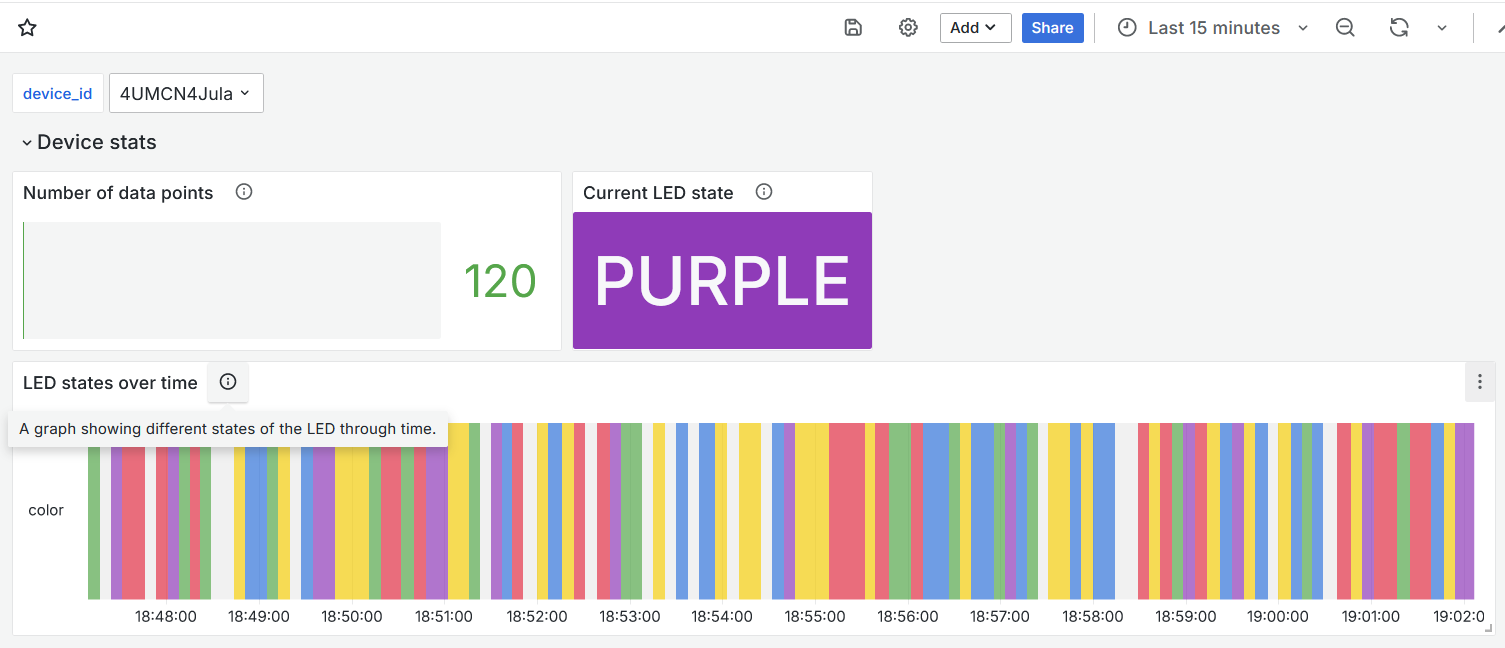
\includegraphics[scale=0.4]{imgs/grafana_device_stats}
	\caption{Prikaz stanja uređaja na Grafani u posljednjih petnaest minuta}
	\label{fig:grafana_device_stats}
\end{figure}

Slika \ref{fig:grafana_device_stats} prikazuje red nadzorne ploče koji sadrži panele stanja uređaja tijekom posljednjih petnaest minuta. Odabran je jedan identifikator uređaja, stoga se prikazuju podaci samo za taj jedan uređaj. Prvi panel prikazuje koliko se ukupno vremenskih točaka nalazi u bazi odabranom vremenskom okviru, drugi prikazuje posljednje zabilježeno stanje LED diode, a posljednji panel prikazuje promjenu stanja LED diode kroz vrijeme. Svako je stanje LED diode označeno prikladnom bojom koristeći preslikavanja koje nudi Grafana. Jedno takvo preslikavanje prikazano je na slici \ref{fig:grafana_value_mapping}. 

\begin{figure}[ht]
	\centering
	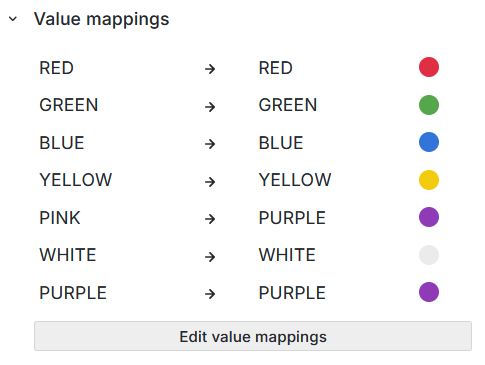
\includegraphics[scale=0.6]{imgs/grafana_value_mapping}
	\caption{Preslikavanje vrijednosti LED dioda na boje}
	\label{fig:grafana_value_mapping}
\end{figure}

Podaci svih prikazanih panela dobiveni su iz kante \textit{esp32state}. Sljedeći je upit korišten za prikaz stanja tijekom vremena. Za vremenski raspon koristi varijable za početak i kraj odabranog vremenskog okvira u Grafani koje nudi \engl{plugin} za bazu InfluxDB. Vrijednost za identifikator uređaja dobiva se iz varijable nadzorne ploče. 

\begin{lstlisting}[caption={Upit za dohvat stanja LED diode u vremenskom okviru}, language=flux]
from(bucket: "esp32state")
|> range(start: v.timeRangeStart, stop: v.timeRangeStop)
|> filter(fn: (r) => r._measurement == "esp32")
|> filter(fn: (r) => r.device_id == "${device_id}")
|> map(fn: (r) => ({ color: r._value, time: r._time }))
\end{lstlisting}

Sljedeće slike prikazuju red sa senzorskim očitanjima. Prva tri panela sa slike \ref{fig:grafana_data_1} prikazuju trenutno izmjerene senzorske vrijednosti, dok drugi panel prikazuje temperaturu tijekom vremena. Isto tako, moguće je primijetiti kako su trenutna mjerenja drukčije obojana. Definirane su granične vrijednosti \engl{thresholds} na temelju kojih se evaluira koje će boje biti panel. Boja simbolizira kritičnost stanja u kojem se uređaj nalazi. Žuta boja signalizira upozorenje, dok crvena predstavlja ozbiljno stanje izmjerene vrijednosti. Ostala dva panela na slici \ref{fig:grafana_data_2} prikazuju vlažnost zraka i vlagu zemlje kroz vrijeme. Na dnu svakog linijskog grafa vidljiv je i serijski broj uređaja, stoga ukoliko je odabrano više uređaja, moguće je i dalje zaključiti koje su vrijednosti vezane za pojedini uređaj. Isto tako, na svakom je panelu odabrana prikladna mjerna jedinica. 

\begin{figure}[ht]
	\centering
	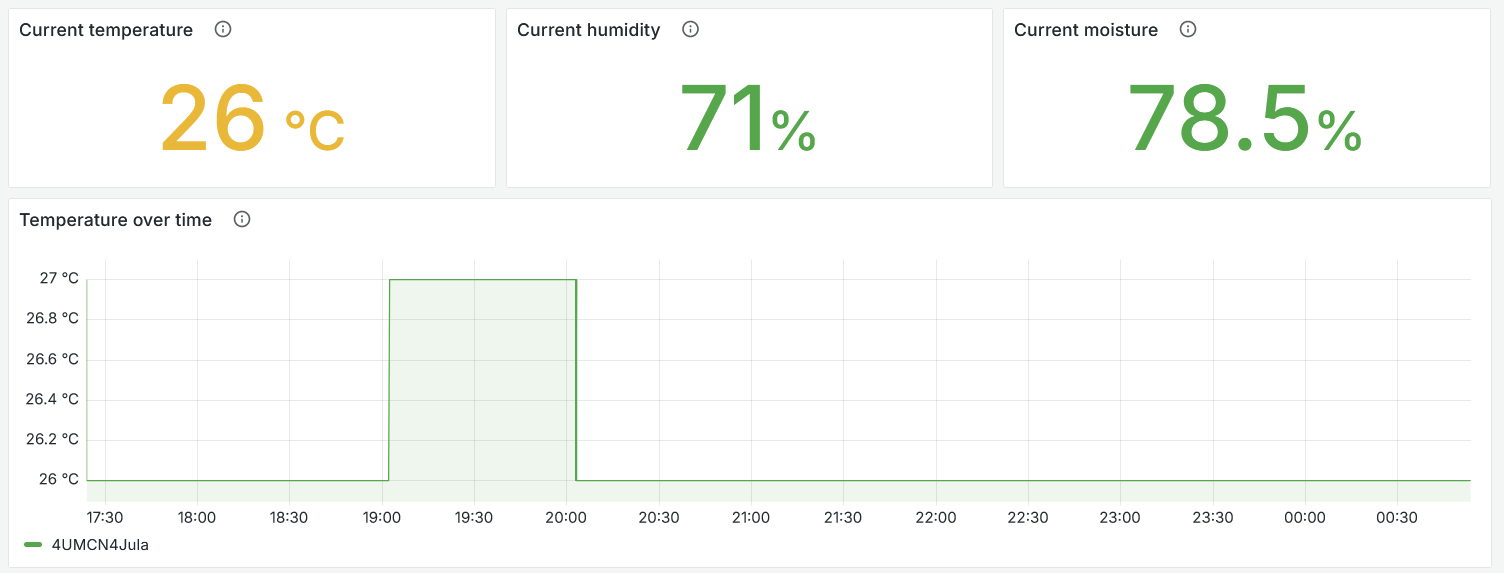
\includegraphics[scale=0.4]{imgs/grafana_data_1}
	\caption{Trenutno izmjerena senzorska mjerenja i temperatura kroz vrijeme}
	\label{fig:grafana_data_1}
\end{figure}

\begin{figure}[ht]
	\centering
	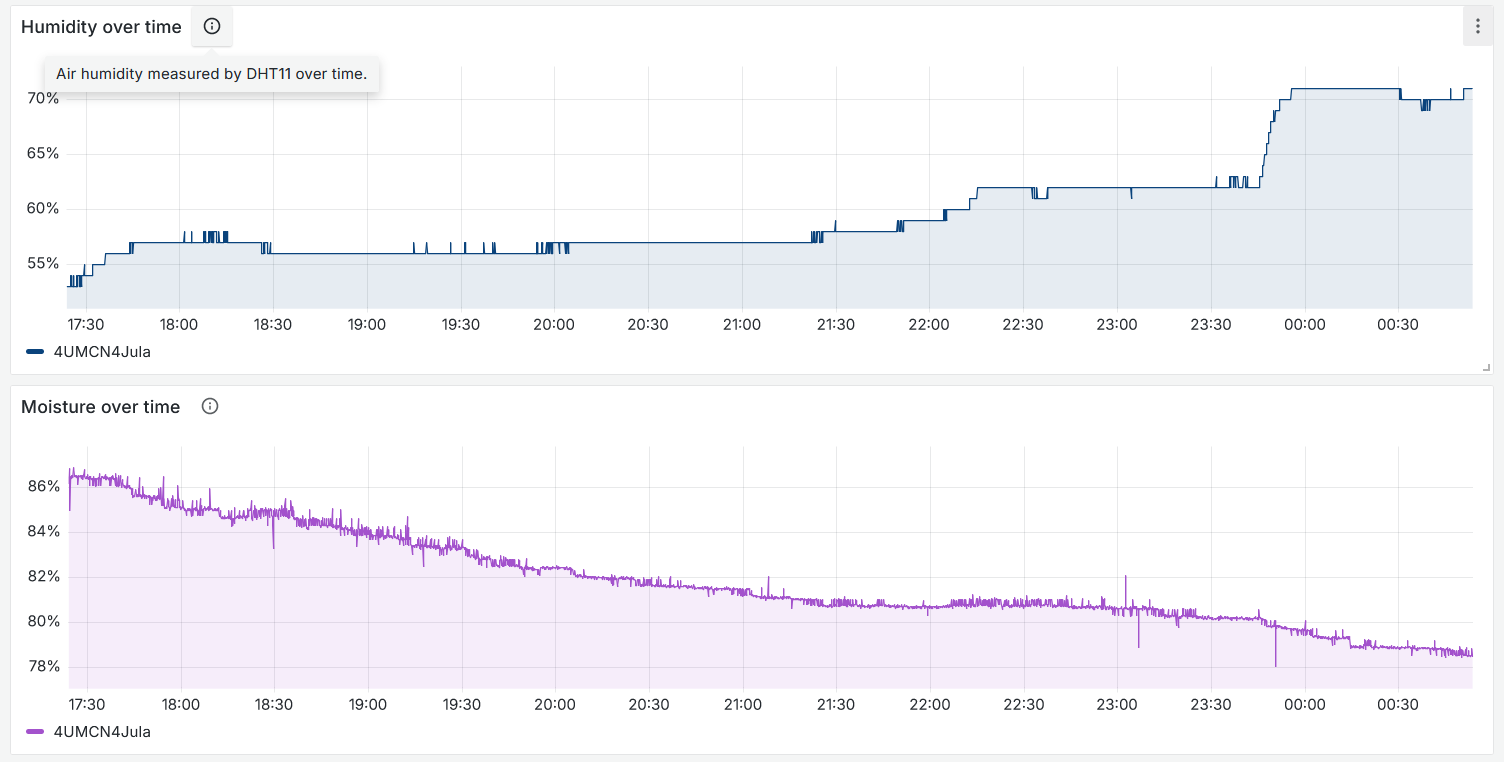
\includegraphics[scale=0.4]{imgs/grafana_data_2}
	\caption{Vlažnost zraka i zemlje kroz vrijeme}
	\label{fig:grafana_data_2}
\end{figure}

Sljedeći programski isječak prikazuje upit za dohvat temperature kroz vrijeme. Kao što je ranije spomenuto, koristi se kanta \textit{esp32data} za izvor podataka o senzorskim očitanjima. Grupiranje po serijskom broju uređaja važno je za točan prikaz podataka. Funkcijom \lstinline|keep()| zadržani su stupci za vrijeme, uređaj te sama vrijednost odabrane temperature, dok su ostali stupci automatski odbačeni.

\begin{lstlisting}[caption={Upit za dohvat temperature}, language=flux]
from(bucket: "esp32data")
|> range(start: v.timeRangeStart, stop: v.timeRangeStop)
|> filter(fn: (r) => r._measurement == "esp32" and r._field == "temperature")
|> filter(fn: (r) => r.device_id == "${device_id}")
|> group(columns: ["device_id"])
|> keep(columns: ["_time", "_value", "device_id"])
\end{lstlisting}

Slika \ref{fig:thresholds} prikazuje ranije spomenute granične vrijednosti za stiliziranje panela. Ove se vrijednosti odnose na panel s trenutnim senzorskim mjerenjem temperature. Srednja granica jest 25°C, dok je kao gornja granica postavljena 30°C. Sve vrijednosti ispod srednje granice označene su zelenom bojom te se smatraju prihvatljivima.

\begin{figure}[ht]
	\centering
	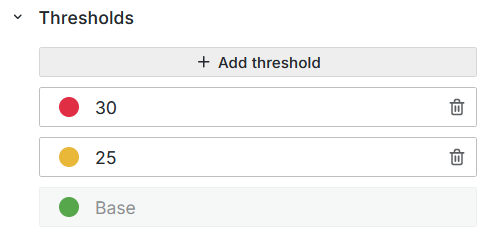
\includegraphics[scale=0.7]{imgs/thresholds}
	\caption{Granične vrijednosti za temperaturu zraka}
	\label{fig:thresholds}
\end{figure}

\subsection{Alarmni sustav}

Korisnici ne prate uvijek stanje uređaja niti očitanja mjerenih senzora, stoga je korisno slati obavijesti korisniku pri svakom neželjenom očitanom stanju. Grafana nudi alarmni sustav \engl{alerting system} koji omogućuje definiranje uvjeta pod kojima se generiraju obavijesti, na temelju podataka i metrika prikupljenih iz različitih izvora podataka. Mogu se kreirati pravila za alarme, postaviti pragovi za različita mjerenja, kao i definirati vremenski intervali za provjeru tih uvjeta. Kada su uvjeti ispunjeni, Grafana može poslati obavijesti putem raznih kanala, od kojih su neki e-pošta, Slack i Discord.  

Alarmni sustav omogućuje proaktivno praćenje performansi i dostupnosti sustava, osiguravajući pravovremenu obaviještenost o potencijalnim problemima. Isto tako, moguće je detaljno konfigurirati obavijesti, uključujući opcije za ponavljanje alarma i kreiranje eskalacijskih lanaca kako bi se osiguralo da obavijest dosegne tražene osobe. Povijest alarma se pohranjuje i može se pregledavati, što olakšava analizu i rješavanje problema \cite{grafana}. 

Dijagram na slici \ref{fig:alerting_system} prikazuje princip rada alarmnog sustava na Grafani. Alarmni sustav Grafane periodički ispituje izvore podataka i procjenjuje uvjet zapisan u pravilu alarma. Ako je uvjet prekršen, uključi se alarm za pojedinu instancu koja je prouzrokovala alarm. Šalju se obavijesti za aktivirane i razriješene alarme direktno kontakt točki ili prolaze notifikacijsku politiku za detaljnije preusmjeravanje. Alarmi se također mogu pridružiti panelima na nadzornim pločama za jednostavniji pregled alarma. 

Grafanin alarmni sustav sastoji se od dvije ključne komponente:
\begin{itemize}
	\item generator alarma: procjenjuje pravila i šalje aktivne ili razriješene alarme primatelju alarma, 
	\item primatelj alarma (\textit{Alertmanager}): prima alarme, odgovoran za njihovo rukovanje i slanje obavijesti.
\end{itemize}

\begin{figure}[ht]
	\centering
	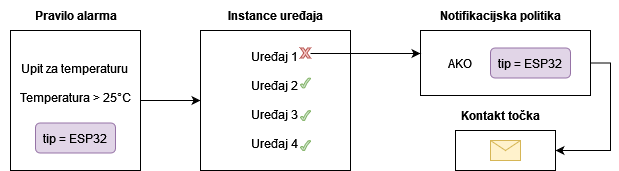
\includegraphics[scale=0.6]{imgs/alerting_system}
	\caption{Princip rada alarmnog sustava na Grafani \cite{grafana}}
	\label{fig:alerting_system}
\end{figure}

U nastavku su pobliže objašnjeni pojmovi ključni za razumijevanje alarmnog sustava.

Pravilo alarma \engl{alert rule} sastoji se od jednog ili više upita i izraza koji odabiru podatke koji se žele mjeriti. Također sadrži uvjet, a to je prag koji pravilo alarma mora ispuniti ili premašiti da bi se aktivirao. Unutar pravila alarma potrebno je odabrati točku kontakta ili notifikacijsku politiku kako bi se odredio način slanja obavijesti. Svako pravilo alarma može proizvesti više instanci, i svako pojavljivanje pravila naziva se alarm. Alarm se generira za svaku vremensku seriju, što je korisno jer se time omogućava praćenje više uređaja samo jednim pravilom. Ako su podaci grupirani po identifikatoru uređaja, alarm će se aktivirati za svaki pojedini identifikator. Pravila se često procjenjuju i njihova se stanja sukladno ažuriraju. Sustav obavještava isključivo o instancama koje ispunjavaju uvjete ili na koji su upravo razriješeni \engl{resolved}. 

Svako pravilo alarma mora imati evaluacijsku grupu te period čekanja \engl{pending period}. Svaka evaluacijska grupa ima razdoblje evaluacije odnosno procjene, i određuje koliko se često alarm procjenjuje. Period čekanja definira koliko dugo uvjet mora biti ispunjen prije nego se alarm pokrene, što smanjuje mogućnost lažno pozitivnih alarma. Period čekanja se isto tako može postaviti na nulu, čime se alarm efektivno pokreće odmah čim je uvjet ispunjen. Slika \ref{fig:alerting_resolved} prikazuje promjene stanja alarma i obavijesti koje se šalju u svakom stanju. Početno je normalno stanje kada uvjet nije ispunjen i alarm nije pokrenut. Kada se uvjet ispuni, alarm prelazi u stanje čekanja \engl{pending} dok period čekanja ne istekne. Na kraju perioda, ako je uvjet i dalje ispunjen, alarm prelazi u aktivno stanje i šalje obavijesti o promjeni stanja. Po završetku ispunjavanja uvjeta, alarm je razriješen i vraća se u normalno stanje, te se šalje obavijest o razrješenju alarma. Isto tako, ako je alarm u stanju čekanja, a uvjet se prestane ispunjavati tokom perioda čekanja, alarm se vraća u početno normalno stanje. 

\begin{figure}[ht]
	\centering
	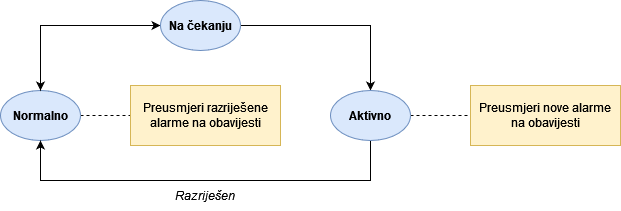
\includegraphics[scale=0.6]{imgs/alerting_resolved}
	\caption{Promjena stanja alarma \cite{grafana}}
	\label{fig:alerting_resolved}
\end{figure}

Notifikacijske politike pružaju fleksibilan način preusmjeravanja obavijesti. One usmjeravaju alarme na točke kontakta pomoću uparivanja oznaka \engl{label matching} s alarma. Notifikacijske politike nisu lista, nego stablasta struktura, čiji je korijen zadana notifikacijska politika te iz nje proizlaze mnoge politike. Svaka politika ima skup oznaka na temelju kojih se uparuje s kontaktnim točkama. Unutar alarma definiraju se oznake koje se nakon aktiviranja alarma uparuju s notifikacijskim politikama. Slika \ref{fig:label_matching} prikazuje princip uparivanja oznaka alarma s notifikacijskim politikama. Što je više oznaka definirano u alarmu, to dublje prolazi u strukturu notifikacijskih politika. Kako bi se odredilo koje notifikacijske politike trebaju rukovati alarmom, oznake se uparuju od početka stabla, odnosno zadane notifikacijske politike. Ona je uparena sa svim alarmima, što sprječava propuštanje preusmjeravanje alarma. Ako se pronađe podudarna politika, sustav nastavlja procjenjivati politike dublje u strukturi redom kojim su navedene. Ako je ugniježđena politika s alarmom, evaluiraju se i njezine podpolitike. Ovaj se proces odvija rekurzivno dok se ne dođe do najdublje politike u strukturi koja se podudara s oznakama alarma. U ovom slučaju, samo politika najdublje u strukturi obrađuje alarm. Ako alarm treba obraditi više politika, treba omogućiti uparivanje sa hijerarhijski srodnim odnosno sestrinskim pravilima na željenoj razini.  

\begin{figure}[ht]
	\centering
	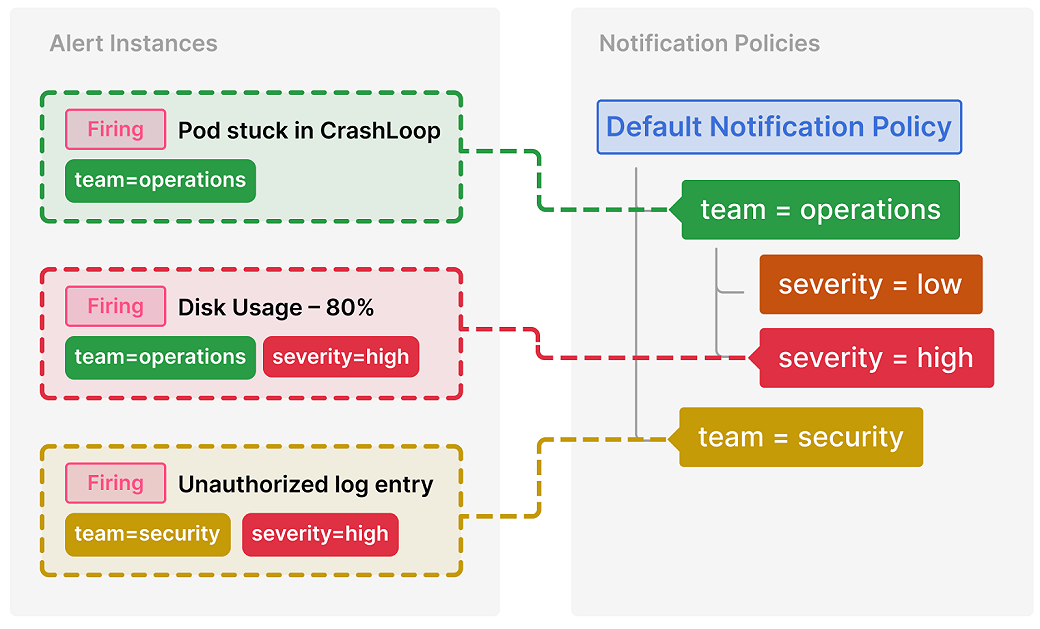
\includegraphics[scale=0.4]{imgs/label_matching}
	\caption{Uparivanje oznaka alarma i notifikacijskih politika \cite{grafana}}
	\label{fig:label_matching}
\end{figure}

Kao što je spomenuto, svaka je notifikacijska politika vezana za jednu točku kontakta \engl{contact point}. Točke kontakta sadrže konfiguraciju za slanje obavijesti o alarmima. To je popis integracija od kojih svaka šalje obavijest na određeni kanal. Grafana pruža integraciju s brojnim sustavima i aplikacijama za slanje pošte ili obavijesti. Unutar svake točke također se definira poruka obavijesti koja se šalje, a može koristiti unaprijed kreirane predloške ili poruku. Moguće je definirati i kontaktnu točku bez ikakve integracije, no u tom slučaju ona ne šalje nikakve obavijesti. Slika \ref{fig:labels_and_notifs} prikazuje vezu notifikacijskih politika i točaka kontakta.

\begin{figure}[ht]
	\centering
	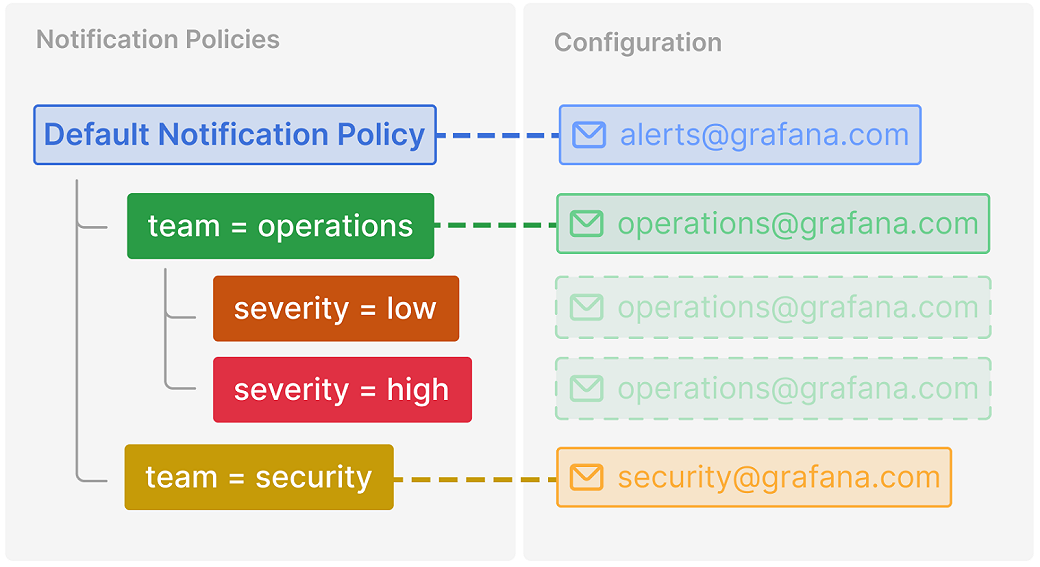
\includegraphics[scale=0.4]{imgs/labels_and_notifs}
	\caption{Uparivanje notifikacijskih oznaka i točaka kontakta \cite{grafana}}
	\label{fig:labels_and_notifs}
\end{figure}

Moguće je kreirati i predloške za slanje poruka u obavijesti. Za kreiranje predložaka koriste se predlošci programskog jezika Go. Naime, primatelj obavijesti odnosno komponenta \textit{Alertmanager} jest aplikacija napisana u programskom jeziku Go, te se kreirani predlošci prosljeđuju toj komponenti i izravno integriraju u njezin izvorni kod. Predlošci pružaju mogućnost definiranja strukture i sadržaja obavijesti o alarmima, čime postaju informativnije i prilagođenije potrebama. Važno je napomenuti kako postavljanjem predloška za točku kontakta sve obavijesti koje dolaze s te točke poprimaju oblik definiran predloškom. 

Predlošci se pišu koristeći sintaksu dvostrukih zagrada \lstinline|{{...}}| koje označavaju mjesta gdje će se dinamički umetnuti sadržaj. Unutar ovih zagrada mogu se koristiti različite naredbe poput varijabli, funkcija, petlji i uvjetnih izraza. Podaci se u predloške ubacuju kroz kontekst koji je struktura ili rječnik podataka proslijeđen predlošku pri njegovu izvršavanju. Unutar primatelja obavijesti, predložak se učitava i obrađuje, nakon čega se izvršava s određenim podacima pomoću posebnih funkcija izvršavanja. Pri izvršavanju, dinamički podaci zamjenjuju odgovarajuće oznake unutar predloška, generirajući konačni izlazni sadržaj. Sustav predložaka omogućuje i definiranje prilagođenih funkcija koje se mogu koristiti unutar predložaka. Ovo omogućuje proširenje funkcionalnosti predložaka dodavanjem specifičnih operacija koje se mogu izvršavati nad podacima, čime se povećava fleksibilnost cijelog sustava predložaka \cite{go_templating}. 

Sljedeći odsječak koda prikazuje primjer jednog predloška u programskom jeziku Go kakav bi se mogao naći u točki kontakta alarmnog sustava Grafane. Unutar definiranog predloška prolazi se po svim generiranim alarmima i za svaki alam iz popisa oznaka odabere se oznaka s ključem \textit{alertname}. Isto tako, provjerava se trenutno stanje alarma i na temelju dobivene varijable generira se ostatak poruke. 

\begin{lstlisting}[caption={Primjer predloška u programskom jeziku Go}, language=go]
{{ define "custom_alert_template" }}
	{{ range .Alerts }}
		This is my alert named {{ index .Labels "alertname" }}
		{{ if eq .Status "resolved" }}
			This alert is resolved.
		{{ else }}
			This alert is currently firing!
		{{ end }}
	{{ end }}
{{ end }}
\end{lstlisting}

Predlošci u jeziku Go prate određenu strukturu, te se varijable predloška mijenjaju podacima iz samog alarma. Sučelje za kreiranje predloška nudi i provjeru napisanog testirajući predložak nad testnim alarmom. Također je moguće verificirati valjanost predloška s podacima iz trenutno aktivnog alarma. Slika \ref{fig:grafana_templating} prikazuje testiranje gornjeg predloška nad kreiranim testnim alarmom. Alarmi su podaci u formatu JSON koji se dinamički učitaju u taj predložak.

\begin{figure}[ht]
	\centering
	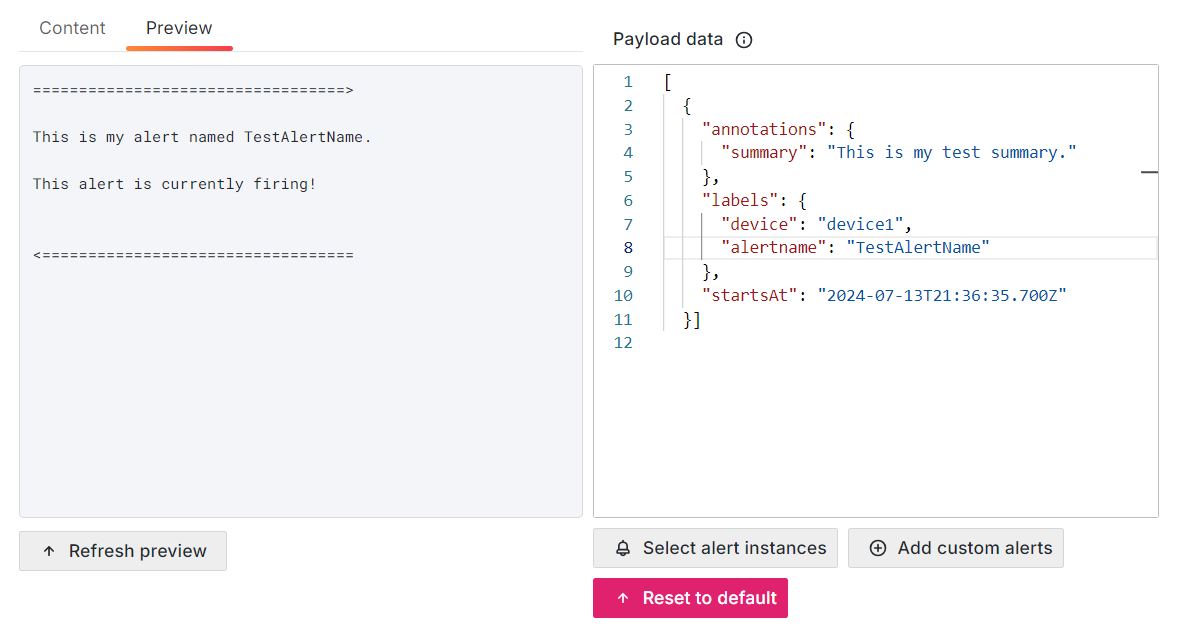
\includegraphics[scale=0.4]{imgs/grafana_templating}
	\caption{Primjer testiranja predloška nad probnim alarmom}
	\label{fig:grafana_templating}
\end{figure}

Za potrebe razvijenog sustava kreirano su dva alarma: alarm za vlažnost tla te alarm kada u bazi nema novih podataka duži vremenski period. Najprije je kreiran alarm kada je u kanti \textit{esp32state} vrlo malo ili nema uopće podataka u posljednjih deset minuta. Alarm je kreiran pomoću sljedećeg upita:

\begin{lstlisting}[caption={Upit za alarm o nedostatku podataka}, language=flux]
from(bucket: "esp32state")
|> range(start: v.timeRangeStart, stop: v.timeRangeStop)
|> filter(fn: (r) => r._measurement == "esp32")
|> group(columns: ["device_id"])
|> count()
|> group(columns: ["device_id"])
|> map(fn: (r) => ({ 
	_value: r._value,
	device_id: r.device_id
}))
|> yield(name: "count")
\end{lstlisting}

Upit je vrlo sličan ranijem upitu za dohvat podatkovnih točaka, no razlika jest što sljedeći upit vraća isključivo broj pronađenih točaka. Ako se u kanti nalazi manje od pet točaka, ili ako ih nema uopće, alarm se aktivira. Također je postavljeno aktiviranje alarma ako upit ne vrati nikakvu vrijednost, ili vrati praznu vrijednost. Evaluacijski period je pet minuta, te uvjet mora biti ispunjen još sljedećih pet minuta kako bi se alarm aktivirao. Slika \ref{fig:alert_rule_esp32state} prikazuje kreirani alarm. Alarmu su dodijeljene dvije oznake: jedna za vrstu uređaja, dok druga definira primatelja alarma. Notifikacijska politika povezuje ovu oznaku sa kontaktnom točkom. Alarm je također moguće utišati na željeni vremenski period. Utišanja alarma \engl{alert silences} stvaraju se na temelju oznaka i imena alarma. Obavezno je definirati trajanje utišanja budući da nije moguće neograničeno utišati alarme. 

\begin{figure}[ht]
	\centering
	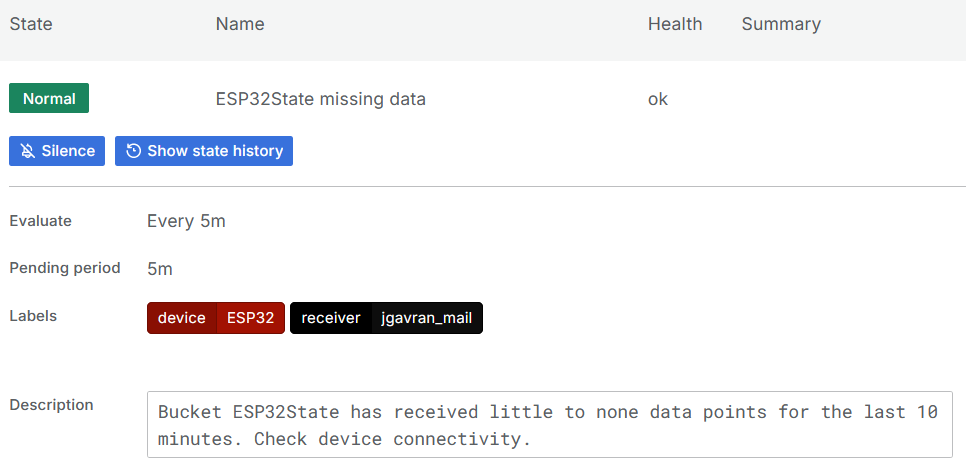
\includegraphics[scale=0.6]{imgs/alert_rule_esp32state}
	\caption{Alarm za podatke koji nedostaju posljednjih deset minuta}
	\label{fig:alert_rule_esp32state}
\end{figure}

Na slici \ref{fig:alert_rule_esp32state_states} nalaze se stanja alarma kroz vrijeme. Vremenski najstarije stanje prikazano je na dnu tablice stanja. Kao što je vidljivo na slici, alarm je bio aktivan određeni vremenski period. Oznaka \textit{Nodata} indikator je da je alarm aktiviran jer upit nije vratio nikakav rezultat, što je također znak da se u kanti ne nalaze nikakvi podaci. Nakon toga je alarm pauziran, čime se vratio u normalno stanje. Nakon toga je ponovno pokrenut, te budući da se u idućih pet minuta u bazi nisu pojavili nikakvi podaci, alarm prelazi u stanje čekanja označeno žutom bojom. Po isteku vremena čekanja alarm se ponovno aktivirao. 

\begin{figure}[ht]
	\centering
	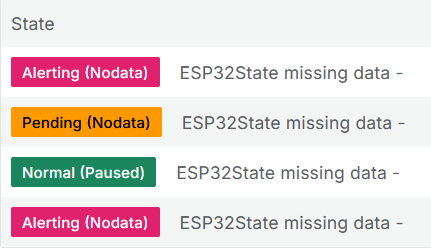
\includegraphics[scale=0.6]{imgs/alert_rule_esp32state_states}
	\caption{Promjena stanja alarma za podatke}
	\label{fig:alert_rule_esp32state_states}
\end{figure}

Slika \ref{fig:notif_policy} sadrži prikaz notifikacijskih politika. Vidljiva je ugniježđena stablasta struktura politika. Isto tako, na dnu se nalazi nova notifikacijska politika koja sve alarme s oznakom primatelja postavljenom na \textit{jgavran\_mail} preusmjerava na kontaktnu toočku \textit{jgavran\_mail}. Ta kontaktna točka sadrži popis adresa e-pošte na koje se šalje obavijest o alarmu. 

\begin{figure}[ht]
	\centering
	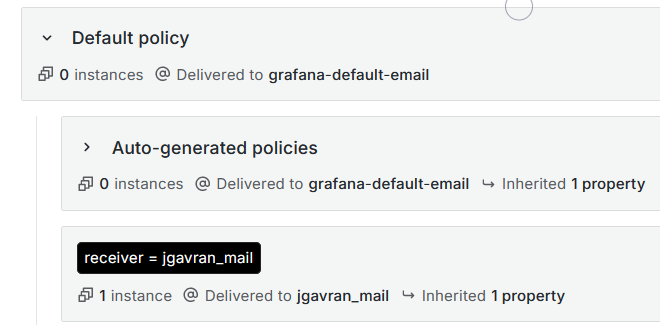
\includegraphics[scale=0.6]{imgs/notif_policy}
	\caption{Popis notifikacijskih politika i pripadajućih oznaka}
	\label{fig:notif_policy}
\end{figure}

Kreirani su predlošci za naslov i tijelo obavijesti alarma. Kao što je ranije opisano, korišteni su predlošci programskog jezika Go. Svaka poruka e-pošte koja se pošalje putem točke kontakta formatirana je na temelju kreiranog predloška. U nastavku su navedeni predlošci za naslov i tijelo poruke. Predložak za naslov je jednostavan, te osim naziva alarma sadrži jedino provjeru je li poslana obavijest o aktivaciji ili razrješenju alarma. S druge strane, predložak za tijelo koristi puno više sadržaja samog alarma za generiranje obavijesti. Na početku samog predloška definirane su varijable za poruku, sažetak i opis alarma. Sve tri varijable su navedene jer postoji mogućnost da će kreirani alarm imati jedno ili pak više od opisnih polja, stoga je važno uzeti u obzir sve opcije. Nakon toga, ovisno o tome postoje li varijable ili ne, uključuju se u predložak. Budući da je alarme moguće pridružiti nadzornim pločama, ako je navedenom alarmu pridružen panel odnosno nadzorna ploča, prikazat će se izravna poveznica na ploču. Nadalje se prikazuju sve oznake definirane u alarmu kao i vrijednosti samih izraza korištenih u alarmu kako bi obavijest bila potpunog sadržaja i kako bi korisnik zaključio je li potrebno brzo reagirati na obavijest.

\begin{lstlisting}[caption={Predlošci za naslov i tijelo obavijesti alarma}, language=go]
{{ define "jgavran_title_template" }}
	{{ range .Alerts }}
		{{if eq .Status "resolved" }}
		[OK] {{ index .Labels "alertname" }}
		{{ else }}
		[FIRING] {{ index .Labels "alertname" }}
		{{ end }}
	{{ end }}
{{ end }}

{{ define "jgavran_body_template" }}

{{ range .Alerts }}

	{{- $message := index .Annotations "message" -}}
	{{- $summary := index .Annotations "summary" -}}
	{{- $description := index .Annotations "description" -}}
	
	{{- if $message }}
	{{$message -}}
	{{ end }}
	{{- if $summary }}
	{{$summary -}}
	{{ end }}
	{{- if $description }}
	{{$description -}}
	{{ end }}
	
	Dashboard: {{ .DashboardURL }}
	Labels:
	{{ range .Labels.SortedPairs -}}
		- {{ .Name }} = {{ .Value }}
	{{ end }}
	Values:
		{{ .ValueString }}
	
{{ end }}

{{ end }}
\end{lstlisting}

Sljedeća slika prikazuje obavijest dobivenu na temelju opisanog alarma koji je preusmjeren na točku kontakta e-pošte i zatim obrađen gornjim predloškom. Iz naslova je moguće vidjeti kako je alarm razriješen, a u samom tijelu nalaze se detaljnije informacije o samom alarmu. 

\begin{figure}[ht]
	\centering
	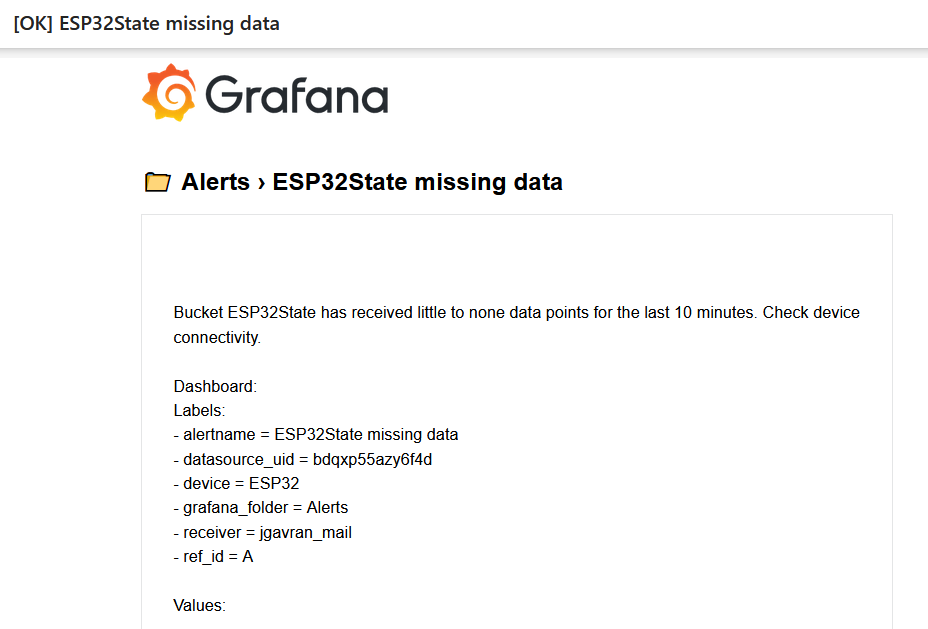
\includegraphics[scale=0.6]{imgs/alert_mail}
	\caption{E-pošta o razriješenom alarmu}
	\label{fig:alert_mail}
\end{figure}

Kao što je već spomenuto, alarmi se mogu pridružiti pojedinim panelima. Tako je kreiran alarm za senzorsko očitanje vlažnosti tla i pridružen je pripadnom linijskom vremenskom grafu. Važno je napomenuti kako se alarmi mogu pridružiti samo panelima koji prikazuju vremenske serije. Upit za vlažnost tla dohvaća samo posljednje vrijednosti za svaki uređaj i u postavkama alarma izraz se evaluira svakih deset sekundi, što je ujedno i minimalno dozvoljeni evaluacijski period. Period čekanja odnosno vremenski okvir u kojem uvjet mora biti ispunjen jest jedna minuta. Periodi su postavljeni tako nisko radi jednostavnijeg testiranja alarma, no nakon provjere valjanosti alarma jednostavno ih je prilagoditi. Kao granica prihvatljivosti vlažnosti zemlje uzeta je vrijednost od 20\%. Na slici \ref{fig:moisture_alert} nalazi se ranije prikazan graf za vlažnost tla kroz vrijeme, no ovaj mu je put pridružen alarm. Ikona srca pokraj naziva panela upućuje da je alarm vezan za njega. Na grafu je vidljivo kako je na početku vlažnost tla jednaka nuli, stoga je poslije prve evaluacije nakon kreiranja alarma alarm promijenio stanje u čekanje, što je označeno okomitom žutom crtom. Nakon isteka perioda čekanja, a vlažnost tla je i dalje ispod dozvoljene vrijednosti, alarm prelazi u aktivno stanje. Aktivacija alarma signalizira se crvenom okomitom crtom. Vlažnost tla je zatim promijenila vrijednost u otprilike 50\%, zbog čega je stanje alarma nakon jedne minute vraćeno u normalno, i to se očituje okomitom zelenom crtom.

\begin{figure}[ht]
	\centering
	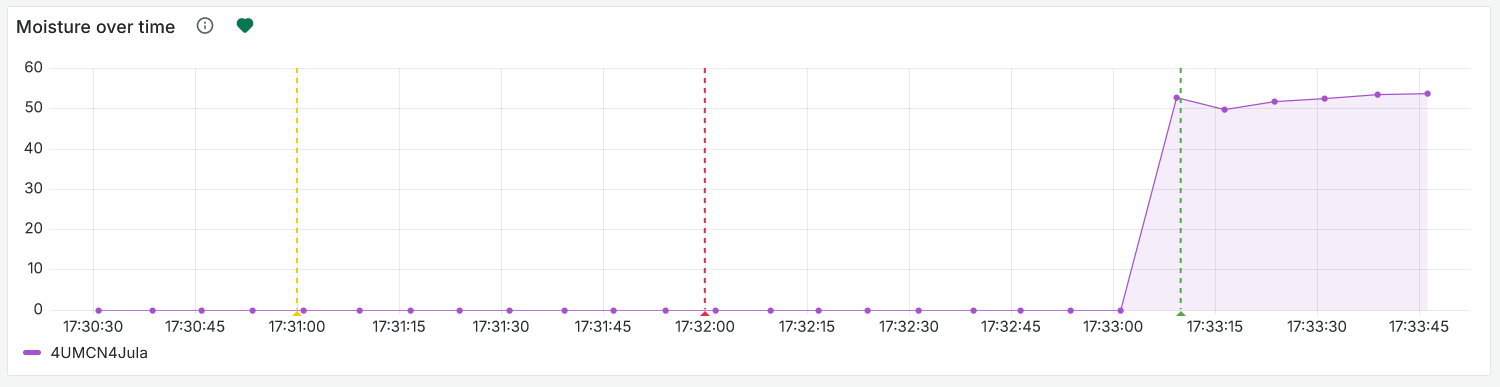
\includegraphics[scale=0.35]{imgs/moisture_alert}
	\caption{Alarm za vlažnost tla kroz vrijeme}
	\label{fig:moisture_alert}
\end{figure}

Sljedeće dvije slike \ref{fig:firing_low_moisture} i \ref{fig:ok_low_moisture} prikazuju obavijesti dobivene pri aktivaciji i razrješenju alarma. Vrijednosti izraza A i B odnose se na strukturu samog alarma. Izraz A jest vrijednost samog upita, dok je izraz B procjena postavljenog uvjeta. Iz prve se obavijesti može vidjeti da je vrijednost izraza A bila jednaka nuli, što je vidljivo i na gornjem grafu. Budući da je uvjet postavljen u izrazu B zadovoljen, odnosno vrijednost izraza A je manja od 20, vrijednost izraza B jednaka je jedinici, što signalizira aktivaciju alarma. S druge strane, u obavijesti razrješenja alarma vrijednost izraza A jednaka je 52.68, što je više od postavljenog uvjeta izraza B, stoga je njegova vrijednost jednaka nuli. 

\begin{figure}[ht]
	\begin{minipage}[t]{0.4\textwidth}
		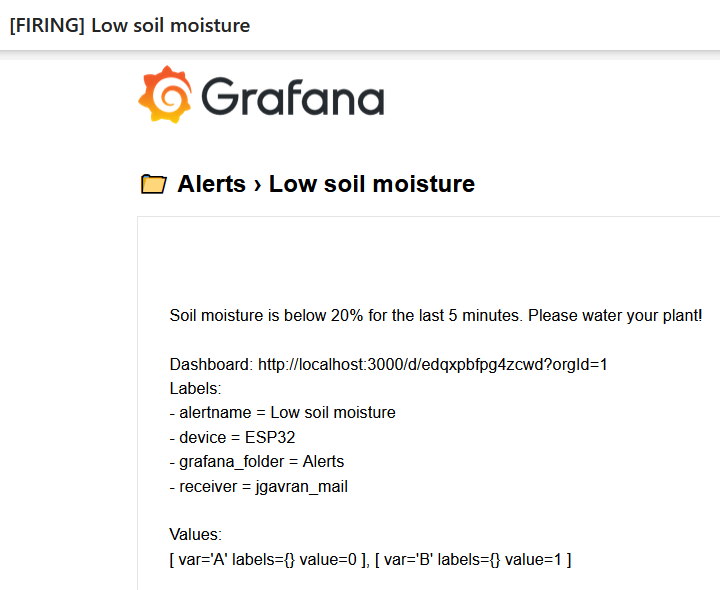
\includegraphics[width=\linewidth]{imgs/firing_low_moisture}
		\caption{Obavijest o aktivaciji alarma niske vlažnosti tla}
		\label{fig:firing_low_moisture}
	\end{minipage}
	\hspace*{\fill}
	\begin{minipage}[t]{0.4\textwidth}
		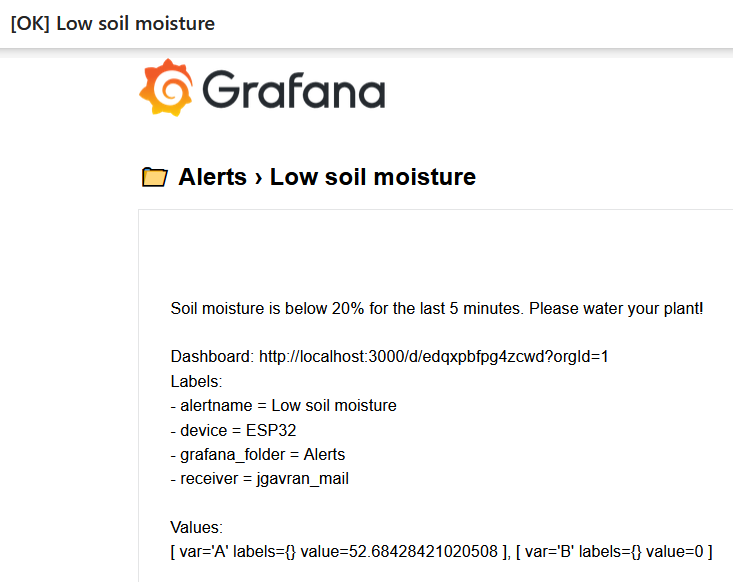
\includegraphics[width=\linewidth]{imgs/ok_low_moisture}
		\caption{Obavijest o razrješenju alarma niske vlažnosti tla}
		\label{fig:ok_low_moisture}
	\end{minipage}
\end{figure}

Alarmi se mogu sukladno napraviti za vlagu i temperaturu zraka. Preporuča se kreirati odvojene alarme za sva senzorska očitanja kako bi imali različite granične vrijednosti. Isto tako, ako korišteni uređaji prate drukčije uvjete gdje su granične vrijednosti različite od postavljenih, moguće je kreirati i alarme specifične uređajima. Potrebno je samo u upit alarma navesti specifičan uređaj nad kojim se ispituju podaci. 

Osim e-pošte, alarmi se mogu preusmjeravati na različite kanale i mobilne aplikacije koje podržavaju obavještavanje. Aplikacije koje se često koriste za slanje obavijesti su PagerDuty i Opsgenie. To su vodeće aplikacije za upravljanje incidentima i obavještavanje koje pomažu organizacijama da odgovore na kritične probleme i smanje vrijeme odgovora na incident. Aplikacije se jednostavno integriraju s različitim sustavima za praćenje i omogućavaju definiranje složenih pravila obavještavanja i automatizaciju eskalacijskih postupak. Osim \textit{push} notifikacijama, aplikacije mogu slati obavijesti i putem SMS poruke te poziva, ovisno o definiranoj eskalacijskoj politici \cite{pagerduty_vs_opsgenie}. Navedene aplikacije mogu se integrirati s Grafanom pomoću API ključa kreiranog u aplikaciji. Tako se obavijesti o promjenama stanja u razvijenom sustavu mogu detaljnije i pozornije pratiti. 

\eject